\chapter{Sicherheitslücken}\label{Sicherheitsluecken}
Damit ein verteiltes System möglichst sicher gestaltet werden kann, ist eine konkrete Analyse des Systems notwendig. Die Analsyse deckt Sicherheitslücken auf und evaluiert welche Angriffe auf welche Systemteile vorgenommen
werden könnten. Um hierfür näheres Verständnis zu erlangen, werden zunächst konkrete Angriffe auf verteilte Systeme definiert und daraus Anforderungen abgeleitet.

\section{Angriffe}

Informationstechnische Systeme werden heute kaum vollständig isoliert eingesetzt. Das beste Beispiel
dafür sind verteilte Systeme. Die Kommunikation zwischen den Systemen findet dabei über lokale und globale 
Netze statt. Dabei wird die globale Vernetzung oft von Tätern für schädliche Aktivitäten missbraucht.
Die Motivation hinter einer solchen Aktivität ist häufig Geld, Sabotage, Einflussnahme oder Informationsbeschaffung. 
Eine genaue Einteilung der Bedrohungen und der dazugehörigen Schutzziele für Systeme in der Informationstechnik sieht so aus:

\begin{tabular}[h]{l|c}
    Bedrohungen & Schutzziele \\
    \hline
    Unbefugter Informationsgewinn & Verlust der Vertraulichkeit \\
    Unbefugte Modifikation von Informationen & Verlust der Integrität \\
    Unbefugte Beeinträchtigung der Funktionalität & Verlust der Verfügbarkeit \\
\end{tabular}


Vertraulichkeit = Informationen werden nur Berechtigten bekannt.
\newline
Integrität = Informationen sind richtig, vollständig und aktuell
oder aber dies ist erkennbar nicht der Fall.
\newline
Verfügbarkeit = Informationen sind dort und dann zugänglich,
wo und wann sie von Berechtigten gebraucht werden.

Bei dem Aufbau eines verteilten Systems sollte stets darauf geachtet werden die Werte 
aufrecht zu erhalten. Eine genauere Beschreibung der Schutzziele wird in \autoref{Sicherheitsdienste} genannt. 
Zur Besseren Beurteilung und Abwehr von Angriffen teilt man diese in verschiedene Kategorien ein,
die jeweils ein Abweichen vom normalen Datenfluss anzeigen.

\begin{figure}[H]
    \centering
    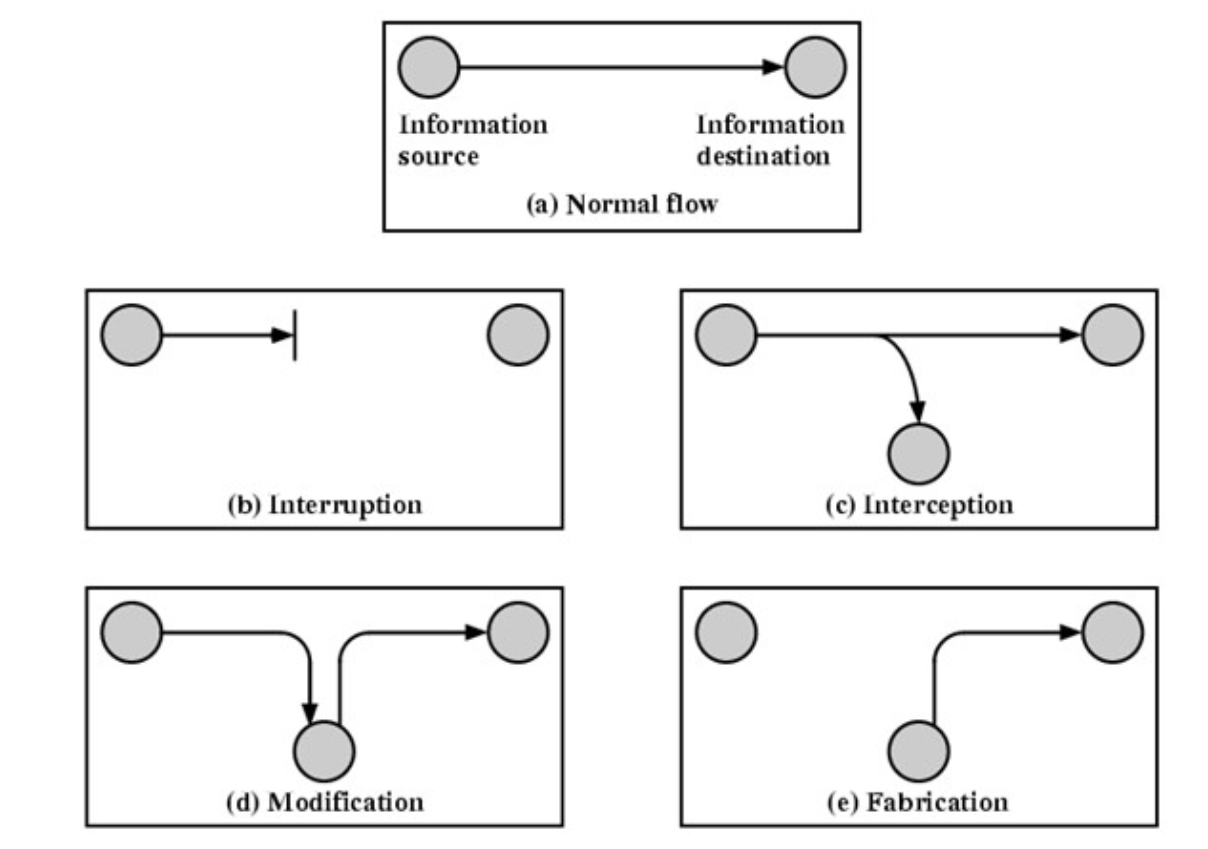
\includegraphics[width=\textwidth]{images/angriffe_pic1.png}
    \caption[Beschreibung für Inhaltsverzeichnis]{Bildbeschreibung} 
    \label{Referenz}
\end{figure} 

\paragraph{Unterbrechungen}
Von einer Unterbrechung wird immer dann gesprochen wenn ein Bestandteil des 
IT-Systems zerstört oder unbrauchbar gemacht wird. Die Angriffe zielen darauf 
ab die Verfügbarkeit des betroffenen IT-Systems zu schwächen. 

\paragraph{Abfangen}
Die oft als \glqq Man-in-the-middle \grqq{} Angriffe bezeichneten Attacken sind dieser 
Kategorie zuzuweisen. Ein nicht berechtigter Benutzer versucht die Vertraulichkeit des 
IT-Systems zu kompromittieren.  

\paragraph{Modifikation}
Von einer Modifikation spricht man immer dann wenn ein Angreifer Zugriff auf einen 
Systemteil gewinnt und auf diesem Daten manipuliert. Diese Angriffsart zielt 
darauf ab die Integrität der Daten zu gefährden. 

\paragraph{Fälschung}
Wenn ein Dritter gefälschte Objekte in eine System einschläust spricht man von 
einer Fälschung. Die Fälschung kompromittiert die Authentizität der Daten. 
Ein Beispiel hierfür wäre sogar bereits die Urkundenfälschung auf einem Computersystem. 

Bei der folgenden Betrachtung von Angriffen auf verteilte Systeme werden die Angriffe jeweils einer 
der aufgeführten Kategorien zugeordnet. 

Der bisher wohl bekannteste Cyber-Angriff wurde 2017 in Form der Ransomeware \glqq WannaCry \grqq{} bekannt.
Mithilfe einer Schwachstelle konnte eine Hackergruppe einen sog. Kryptotrojaner über das Netzwerk
auf sehr viele IT-Systeme verteilen. Besonders interessant in dem Zusammenhang mit verteilten Systemen ist 
das Vorgehen des Trojaners in Unternehmen und Institutionen wir bspw. Krankenhäusern. 
In einigen Krankenhäusern wurden alle Geräte, einschließlich Medizinisches Equipment von 
der Schadsoftware verschlüsselt. 
Die Art der Implementierung des Exploits unterschied sich insofern von anderen Verschlüsselungsprogrammen, 
dass der Benutzer keinen Fehler machen musste um betroffen zu sein. 
Der Virus wurde weder durch einen Word Macro, noch einen verdächtigen Link auf den Computer übertragen. 
Besonders bei großen Unternehmen ohne die nötigen Sicherheitsmaßnahmen wurde großer Schaden angerichtet. 
Teilweise musste bei solchen Fällen die Produktion gestoppt werden, was zu einem enormen wirtschaftlichen 
Schaden geführt hat. 
Ein Solcher Angriff zielt auf die Kompromittierung der Verfügbarkeit und Integrität der Daten des 
Zielsystems ab und sorgt somit für eine Unterbrechung- und Modifikation des normalen Datenflusses. 
\\\\
Ein ebenfalls sehr bekanntes Beispiel für einen Cyber-Angriff ist die Malware \glqq Stuxnet. \grqq{}
Das Ziel des Angriffs war es die Leittechnik zur Urananreicherung im Iran außer Kraft zu setzen. 
Dem Wurm war es möglich, sich über USB-Sticks unbemerkt sogar auf Computersysteme ohne Internetzugang 
auszubreiten. Gerieht die Schadsoftware auf einen Rechner der mit einer bestimmten Maschinensteuerung 
verbunden war, programmierte er diese automatisiert um. Das primäre Ziel des Computervirus bestand darin 
die Verfügbarkeit des Zielsystemes zu kompromittieren was zu einer Unterbrechung des normalen Datenflusses führte. 
\\\\
Die Gefahren von Cyberattacken sind sehr umfangreich die hohe Komplexität der Schadsoftware ist der 
Grund warum man nie von einem vollständigig sicheren System sprechen kann. 
Von dem Bundesamt für Sicherheit in der Informationstechnik (BSI) sind einige Interessante Fakten darüber veröffentlicht worden: 
\begin{itemize}
    \item Etwa alle zwei Sekunden erscheint ein neues Schadprogramm bzw. eine neue Variante
    \item Pro Minute werden ca. 2 digitale Identitäten in Deutschland gestohlen
    \item Pro Tag werden etwa 4-5 geziehlte Trojaner im Regierungsnetz entdeckt
    \item Pro Monat werden etwa 40.000 Zugriffsversuche aus dem Regierungsnetz auf schädliche Websiten blockiert
\end{itemize}


\section{Anforderungen an verteilte Systeme}
Um die Sicherheit im verteilten System gegen die möglichen Angriffe zu schützen müssen einige Anforderungen erfüllt werden. In diesem Abschnitt sollen
konkret die Sicherheitsanforderungen an die verteilten Systeme näher betrachtet werden. Um ein verteiltes System möglich sicher zu gestalten muss eine konkrete Sicherheitsanalyse vorgenommen werden. Hierbei werden alle möglichen Sicherheitslücken und Angriffspunkte aufgedeckt. 
Entsprechend müssen Lösungen und Sicherheitsmechanismen erarbietet und implementiert werden. Da die konkreten Anforderungen an ein verteiltes System sehr unterschiedlich sind und von der konkreten Art des Systems abhängt, werden hier nur einige konkrete Beispiele genannt.
\\\\
Zunächst ist es wichtig, dass das System die Daten der Benutzer vor Angreifern schützt, um Missbrauch zu verhindern. Hierzu zählen beim Beispiel Onlineshops Anmelde- oder Kontodaten. Die Daten und deren Übertragung
schützt ein Zertifikat.
\newline
Weiterhin müssen die Daten des Systems entsprechend ihrer Klassifizierung (öffentlich oder privat) verfügbar gemacht werden. Alle Benutzer werden passend autorisiert und erhalten Zugang zu den ihnen zugänglichen Informationen. Besonders sicher und gut autorisiert müssen dabei die Administratoren werden.
Bei einem Windkraftwerksystem soll beispielsweise nur der Instandhalter und der Manager Zugriff auf das gesamte System bekommen. Alle anderen Arbeiter erhalten nur Zugriff zu dem Teilsystem, welches sie für ihre Arbeit benötigen.
 Änderungen die die Benutzer vornehmen
werden getracked und nachvollziehbar dokumentiert. Auch ein Monitoring über die Systeme muss erfolgen, sodass ein Ausfall schnell erkannt und ein möglicher Unterbrechungs-Angriff verhindert werden kann.
Allgemein muss die Oberfläche so sicher wie möglich gestaltet werden. Weiterleitungen auf andere Seiten und Dienste sollten sicher sein, ebenso muss der Kunde vor Maleware die über das System
übertragen werden kann geschützt werden.
Weiterhin ist neben dem Schutz der Daten auch die Sicherheit der Kommunikation zwischen der Software und dem Kunde wichtig. Dies betrifft zum Beispiel das Senden von E-Mails an den Benutzer. Die Daten werden oft ungescihert
oder unvalidiert versendet. 
Zur Vermeidung von Fälschungen in der Datenhaltung muss das System gewissen Verschlüsselungsmechanismen bereitstellen. 






